\documentclass[a4paper,10pt]{article}
\usepackage[utf8]{inputenc}
\usepackage{amsfonts,amsmath,amssymb,amsthm,amstext,latexsym}
\usepackage{subfig}
%\usepackage{mathdots}
\usepackage{url}
\usepackage{multirow}
\usepackage{tikz}
\usetikzlibrary{calc}
\usetikzlibrary{arrows,shapes}
\usetikzlibrary{patterns,snakes}
\newtheorem{theorem}{Theorem}
%opening
\title{Approximating a Multi-Grid Solver}
\author{Valentin Le Fèvre}

\begin{document}

\maketitle

\section{Introduction}

The multi-grid algorithms are a class of linear system solvers.
The idea is to restrict and interpolate vectors and matrices to smaller spaces to have easier problems to solve, that is, problems that we can solve in much less time than the original one.

This report will investigate the different trade-offs between accuracy and execution time for multi-grid algorithms.
We will focus on a parallel implementation of a multi-grid solver, BoomerAMG~\cite{boomerAMG}, implemented in the HYPRE library~\cite{Falgout2002}.

\section{Definitions}

\begin{itemize}
 \item A system of equations is represented by the following equation: $Ax=b$, where $A \in \mathcal{M}(\mathbb{R})^{n\times n}$ and $b \in \mathcal{\mathbb{R}}^n$ are given and
 $x \in \mathbb{R}^n$ is the unknown. The \emph{exact} solution of this system will be denoted by $\widetilde{x}$.
 \item A level is an integer between $1$ and $L$. Level $1$ will be called the finest level, and level $L$ will be called the coarsest level.
 \item The restriction of $A$ (or $b$ or $x$) to level $l$ will be denoted by $A^l$ (or $b^l$ or $x^l$). We have $A^1 = A$ (and $b^1=b,x^1=x$).
 \item We define a set of $L-1$ restriction matrices $R_1,\dots,R_{L-1}$ such that $R_l b^l = b^{l+1}$. We also define some prolongation matrices $P_1,\dots,P_{L-1}$ such that $P_{l}b^{l+1} = b^l$.
 In other words, we have $P_l = {R_l}^{-1}$ and we build the $A^l$ matrices as follows: $A^{l+1} = R_l A^l P_l$.
 \item We denote by $e^l$ the error at level $l$, that is the vector such that $x^l + e^l = \widetilde{x^l}$, that is to say $\widetilde{x^l}-x^l$.
 We also define the residual at level $l$, $r^l = b^l - A^lx^l$. As $b^l = A^l\widetilde{x^l}$, we can also write $r^l = A^le^l$.
 \item We derive the relative residual norm at any step $i$ in the algorithm
 by the norm of the residual at this step, $||b^l - A^lx^l_i||$, divided by the norm of the initial residual, $|| b^l - A^lx^l_0||$.\\ We also define the notion of \emph{tolerance}
 as an real value between 0 and 1, which is a threshold for stopping an algorithm. In multi-grid algorithms, this threshold will be on the residual norm.
 \item We call relaxation a step of an iterative method for solving linear systems (such as Jacobi, Gauss-Sneidel, \dots). Formally, for a vector $x \in \mathbb{R}^n$, it represents the computation of
 $x \leftarrow Mx + c$ where $M \in \mathcal{M}(\mathbb{R})^{n\times n}$ and $c \in \mathcal{\mathbb{R}}^n$ and are defined depending on the method used.
\end{itemize}

\section{How it works}

  The goal of the algorithm is to improve the efficiency of iterative methods. Indeed, the choice of the starting vector $x$ on which to apply relaxations has consequences on the convergence
  time of the solver, and depending on the system to solve, the convergence of factor (related to the matrix $M$) can be close to 1.\\
  Here the idea is to do some relaxations and then correct the value of $x$ by adding it the corresponding error term. However, this error term cannot be computed easily (otherwise,
  solving the problem would be done by computing the error term and adding it to $x$). Multi-grid solvers instead use recursion to compute the error term. The stopping parameter for the
  recursion will be determined by decreasing the sizes of vectors and matrices (thus loosing on precision but saving time).
  Formally, we can sum up the algorithm as follows:
  
  MG$(l,x,f,\alpha_1,\alpha_2)$:
  \begin{itemize}
    \item If $l = L$, return $x = {A^L}^{-1} f$ (exact solve);
    \item Else:
    \begin{enumerate}
      \item Relax $x$ $\alpha_1$ times using an iterative method (matrix $A^l$, right hand side $f$);
      \item $r \leftarrow R_l ( f - Ax )$;
      \item $y \leftarrow 0$:
      \item MG$(l+1,y,r,\alpha_1,\alpha_2)$;
      \item $e \leftarrow P_{l} y$;
      \item $x \leftarrow x+e$;
      \item Relax $x$ $\alpha_2$ times using an iterative method (matrix $A^l$, right hand side $f$);
   \end{enumerate}
  \end{itemize}
  The algorihtm is then executed by setting $x^l \leftarrow 0$ and then executing MG$(1,x^l,b^l,\alpha_1,\alpha_2)$.

  Then several ways of modifying the algorithm appear:
  \begin{itemize}
   \item Which iterative method to use?
   \item Do we want only one recursion or more?
   \item How many times do we need to apply the algorithm?
   \item How to determine good $\alpha_1$ and $\alpha_2$ parameters?
   \item How many levels should be defined?
  \end{itemize}

  In all what follows the iterative method chosen is an hybrid Jacobi/Gauss-Seidel method. The number of levels used will not be studied.
  
\section{Comparison of existing strategies}

  In this section, we will compare different types of cycles and study how the number of relaxation steps influence the convergence of the algorithm.
  
  We will consider 2 types of cycles: the V-cycle and the W-cycle. The V-cycle is actually the algorithm previously described. The W-cycle looks the same but instead of having two parameters
  $\alpha_1$ and $\alpha_2$ we add a new $\alpha_3$ parameter. It will represent the number of relaxation steps done after a second recursive call. In terms of algorithm it is the same
  algorithm as the V-cycle but the bullets 2 to 7 are repeated. We call these cycles V-cycle and W-cycle because of how we can draw them if we represent each time relaxations are done
  at a level by a point (see Figure~\ref{fig.cycles}). It is possible to define other types of cycles by adding more and more repeats of these steps (do $k$ times those steps) to generalize
  the notion of cycle to a $k$-cycle (where a V-cycle is a $1$-cycle and a W-cycle is a $2$-cycle).
  
 \begin{figure}
 %\resizebox{\linewidth}{4cm}{
 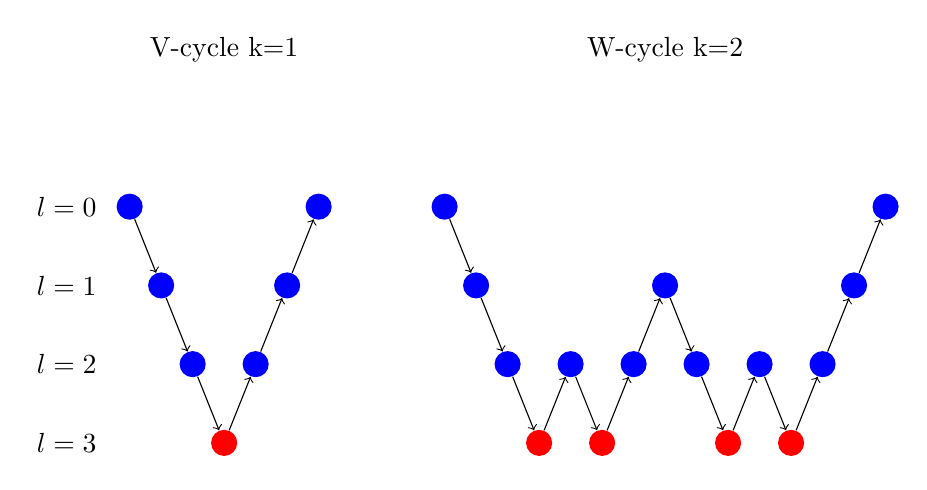
\begin{tikzpicture}
 
 
\begin{scope}[xscale=2/5]

  \node (sh) at (-5,3) { $l=0$ };
  \node (shh) at (-5,2) { $l=1$ };
  \node (shhh) at (-5,1) { $l=2$ };
  \node (shhhh) at (-5,0) { $l=3$};
  
  \node (title) at (0,5) { V-cycle k=1};
  \node (title2) at (14,5) {W-cycle k=2};

    \node[circle,fill=blue] (a) at (-3,3) { };
    \node[circle,fill=blue] (b) at (-2,2) {};
    \node[circle,fill=blue] (c) at (-1,1) {};
    \node[circle,fill=red] (d) at (0,0) {};
    \node[circle,fill=blue] (e) at (1,1) {};
    \node[circle,fill=blue] (f) at (2,2) {};
    \node[circle,fill=blue] (g) at (3,3) {};
    
    \draw[->] (a) -- (b);
    \draw[->] (b) -- (c);
    \draw[->] (c) -- (d);
    \draw[->] (d) -- (e);
    \draw[->] (e) -- (f);
    \draw[->] (f) -- (g);
    
    \node[circle,fill=blue] (aa) at (7,3) { };
    \node[circle,fill=blue] (ab) at (8,2) {};
    \node[circle,fill=blue] (ac) at (9,1) {};
    \node[circle,fill=red] (ad) at (10,0) {};
    \node[circle,fill=blue] (ae) at (11,1) {};
    \node[circle,fill=red] (af) at (12,0) {};
    \node[circle,fill=blue] (ag) at (13,1) {};
    \node[circle,fill=blue] (ah) at (14,2) {};
    \node[circle,fill=blue] (ai) at (15,1) {};
    \node[circle,fill=red] (aj) at (16,0) {};
    \node[circle,fill=blue] (ak) at (17,1) {};
    \node[circle,fill=red] (al) at (18,0) {};
    \node[circle,fill=blue] (am) at (19,1) {};
    \node[circle,fill=blue] (an) at (20,2) {};
    \node[circle,fill=blue] (ao) at (21,3) {};
    
    \draw[->] (aa) -- (ab);
    \draw[->] (ab) -- (ac);
    \draw[->] (ac) -- (ad);
    \draw[->] (ad) -- (ae);
    \draw[->] (ae) -- (af);
    \draw[->] (af) -- (ag);
    \draw[->] (ag) -- (ah);
    \draw[->] (ah) -- (ai);
    \draw[->] (ai) -- (aj);
    \draw[->] (aj) -- (ak);
    \draw[->] (ak) -- (al);
    \draw[->] (al) -- (am);
    \draw[->] (am) -- (an);
    \draw[->] (an) -- (ao);
    \end{scope}
    
 \end{tikzpicture}
 \caption{V-cycle and W-cycle on 4-level grid.}
 \label{fig.cycles}
\end{figure}

A strategy will be composed of a type of cycle (V or W) and a number of relaxation steps $\alpha$. The default implementation of BomerAMG does not allow to have different values
for $\alpha_1,\alpha_2,\dots$ so we set them all to this value $\alpha$. We consider a total of 8 different stragies represented in Table~\ref{table.strat1}.
To compare the different strategies using the BoomerAMG algorithm, we run the algorithm on a predefined matrix of size $512000 \times 512000$ for every
value of maximum number of iterations (i.e. number of cycles) from 1 to 100 and with a required tolerance of $0$ (meaning
that the algorithm will stop when the result is exact or the maximum number of iterations is reached). We measure for each experiment the final relative residual norm and the execution time. Each experiment is run 10 times to have an accurate average execution time.
The results are presented on Figure~\ref{fig.first_tests}.

\begin{table}

\begin{center}
 \begin{tabular}{|c|c|c|c|c|c|c|c|c|}
   \hline
   Type of cycle & V & V & V & V & W & W & W & W \\
   \hline
   $\alpha$ & 1 & 2 & 3 & 10 & 1 & 2 & 3 & 10 \\
   \hline
 \end{tabular}
\end{center}
 \caption{8 strategies.}
 \label{table.strat1}

\end{table}


\begin{figure}
  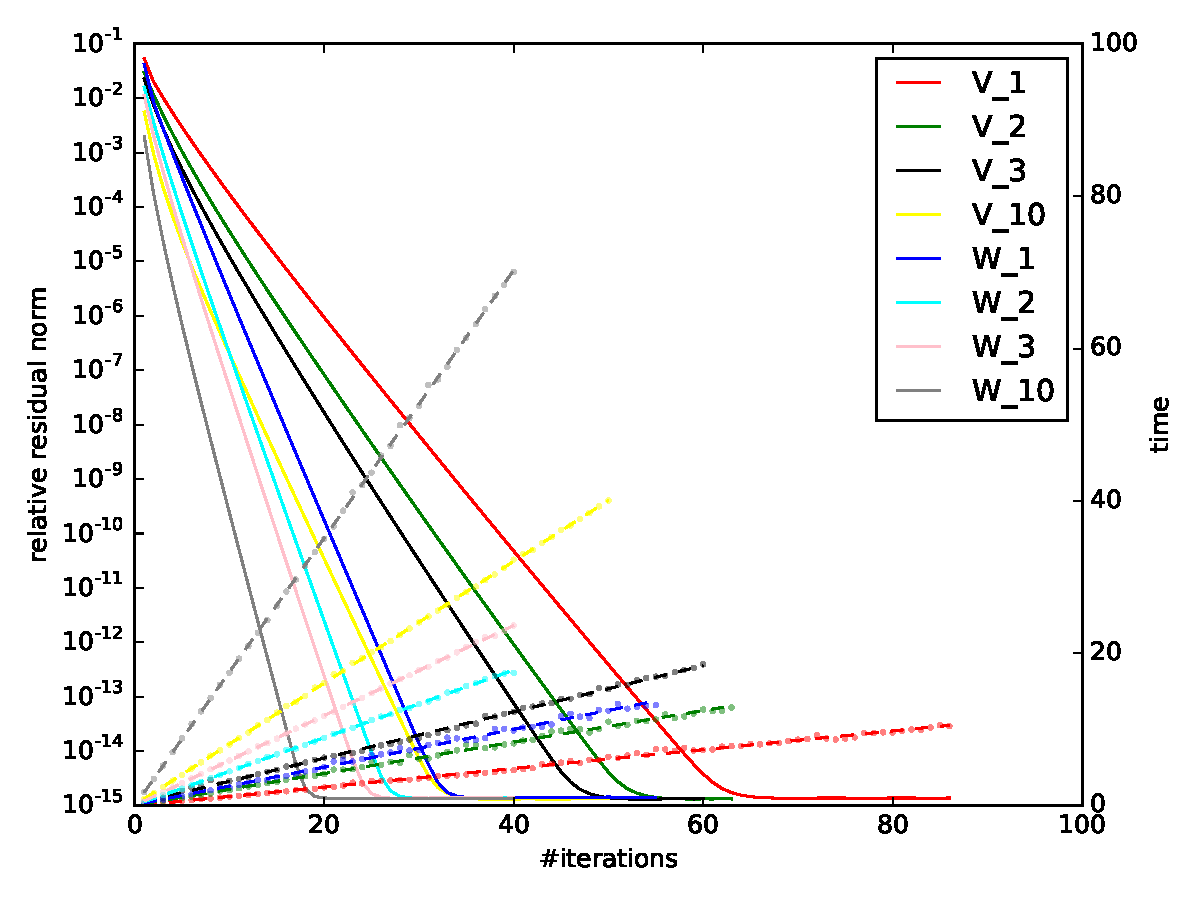
\includegraphics[width=0.49\linewidth]{figs/convergence_1.pdf}
  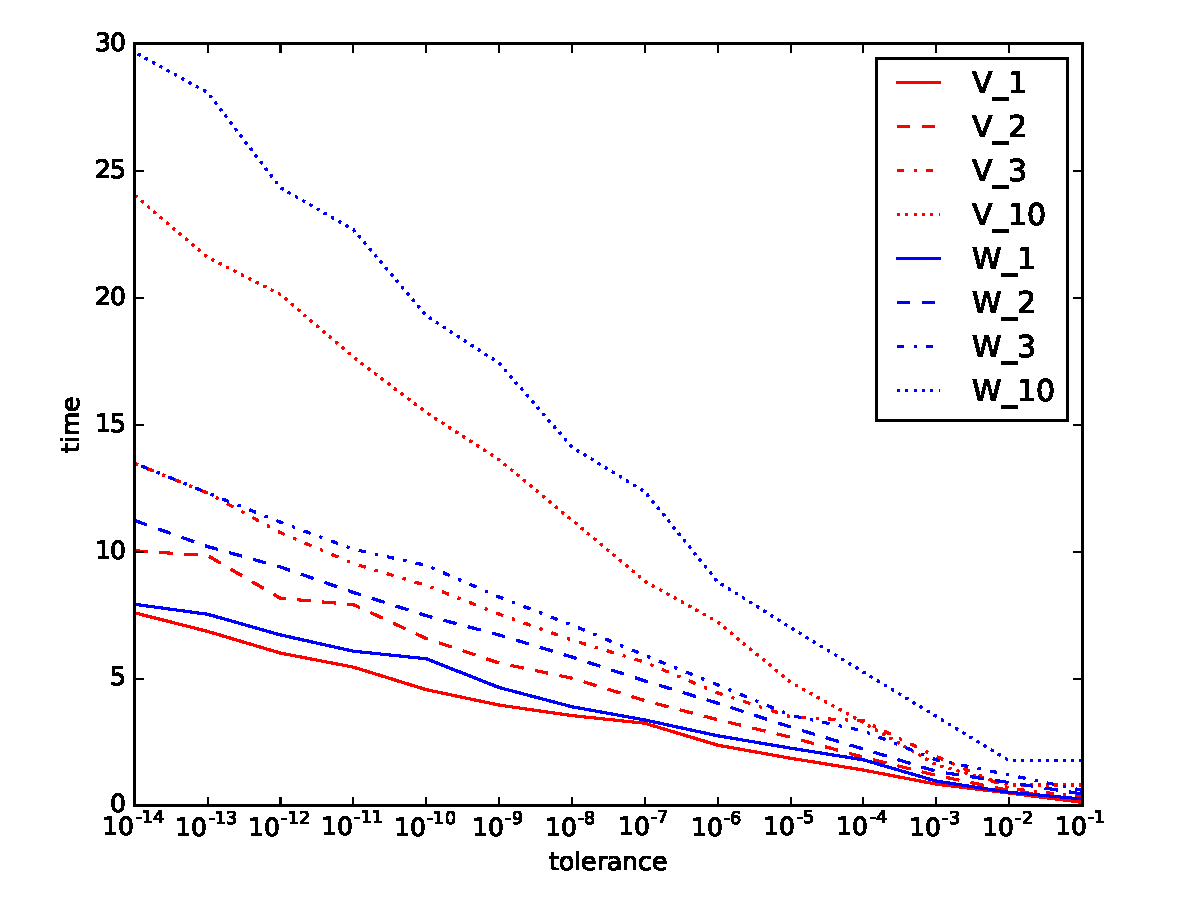
\includegraphics[width=0.49\linewidth]{figs/time_convergence.pdf}
  \caption{Execution time and final residual norm of the 8 strategies.}
  \label{fig.first_tests}
\end{figure} 

What we can observe is that, as expected, increasing the number of relaxation steps or complexifying the cycle increases the overall time to do one cycle. However, it converges in less iterations.
We see on the second figure that actually, for a given precision, the simple V-cycle with only 1 relaxation at each step is the fastest way to reach it, followed closely by the W-cycle with $\alpha=1$.\\
The conclusion is that relaxation steps seem to be too costly for the accuracy they grant. It is better to increase the complexity of your cycle or do more cycles, thus more moves in the grid, than doing more relaxation steps. This at least proves
that multi-grid is a good alternative to classic iterative methods.

\section{Improving the baseline}

\subsection{Symmetric strategies}
Following these results, we can wonder how to improve the efficiency of the simple V-cycle with 1 relaxation step.
The first step is to analyze the time spent in the different parts of a cycle. We measure the time spent doing a relaxation at each level and the time spent computing the next linear system
(when going down in the grid) or the time spent computing the error term (when going up in the grid). The values where measured for a problem of size 512000 with a 8-level grid and are presented
in Table~\ref{table.measures}, along with some information on the matrix used at the corresponding level.

\begin{table}
  \resizebox{\linewidth}{!}{
 \begin{tabular}{|c|c|c|c|c|c|c|}
 \hline
 Level & Matrix size & Non-zero & Relax (down) & Relax (up) & Matvec (down) & Matvec (up) \\
 \hline
  0 & 512,000 & 4,042,520 & 20 ms & 20 ms & 15 ms & -\\
 \hline
  1 & 256,000 & 6,475,239 & 20 ms & 25 ms & 12 ms & 4 ms\\
 \hline
  2 & 58,893 & 2,000,513 & 8 ms & 8 ms & 3 ms & 2 ms\\
 \hline
  3 & 14,285 & 788,509 & 2 ms & 2 ms & 1 ms & 0.7 ms\\
 \hline
  4 & 4,238 & 386,333 & 1 ms & 1 ms & 0.5 ms & 0.2 ms\\
 \hline
  5 & 609 & 53,493 & 0 ms & 0 ms & 0 ms & 0 ms\\
 \hline
  6 & 69 & 2,873 & 0 ms & 0 ms & 0 ms & 0 ms\\
 \hline
  7 & 2 & 4 & 0 ms & - & - & 0 ms\\
 \hline
 \end{tabular}
 }
 \caption{Approximate times spent in the different parts of a V-cycle with $\alpha=1$.}
 \label{table.measures}
\end{table}
 In practice, we notice that the number of non-zero entries in the input matrix is correlated to the average time of a relaxation at a given level. Most importantly, in this example we see that, overall,
 the relaxation represents $\approx66\%$ of the total cost of a V-cycle (while the matrix-vector multiplications are only $\approx30\%$) and that the two first levels are from far the most expensive ones.
 With this information, there are two ideas: (i) adding more relaxations in the last levels because it is almost free or (ii) removing some relaxations in the first levels to reduce the computational cost.
 
 The following 4 strategies were then tested on this same matrix.
  \begin{itemize}
   \item \emph{Fast} : no relaxation at level 2.
   \item \emph{Fast2} : 10 relaxations at level $L-2$.
   \item \emph{Fast3} : 2 relaxations at levels $L-2,L-4,\dots,3$.
   \item \emph{Fast4} : no relaxation at level 3.
  \end{itemize}
  The strategy \emph{Fast} aims at reducing the cost of the cycle by removing the penultimate relaxation (hoping the accuracy lost at this point will be compensated by the relaxation at level 0) which is very costly.
  The strategy \emph{Fast4} is a softer version of \emph{Fast} where the relaxation at level 3 is removed, reaching less improvement of the overall execution time but being more easily compensated by the two relaxations at level 1 and 2.\\
  The strategy \emph{Fast2} executes a lot of relaxations at level $L-2$, because it should not increase by much the execution time of the V-cycle. Why choose $L-2$ level instead of $L$ or $L-1$?
  This because the relaxation at level $L$ is actually a direct solve. Thus, the error term is almost exact at level $L-1$, because the only source of error
  comes from the interpolation of $e^L$ (which is exact) into $e^{L-1}$. This is why, we might expect better results by adding relaxations at level $L-2$.
  The last strategy \emph{Fast3}, pushes this idea one step further. If we assume that doing more than one relaxation gets an really accurate error estimation at level $l$, then
  at level $l-1$ we do not need to correct a lot by doing more relaxations. However at level $l-2$ we have been through 2 interpolations since last good estimation of the error vector, hence increasing the number of relaxations again.
  As we still want not to increase the execution time a lot we stop this recursion for the first levels as they are the two most costly relaxations.
  
  In Figure~\ref{fig.newstrat_small}, we present the results of these 4 strategies on a smaller matrix of initial size 64,000 with only a 6-level grid.
  
  \begin{figure}
  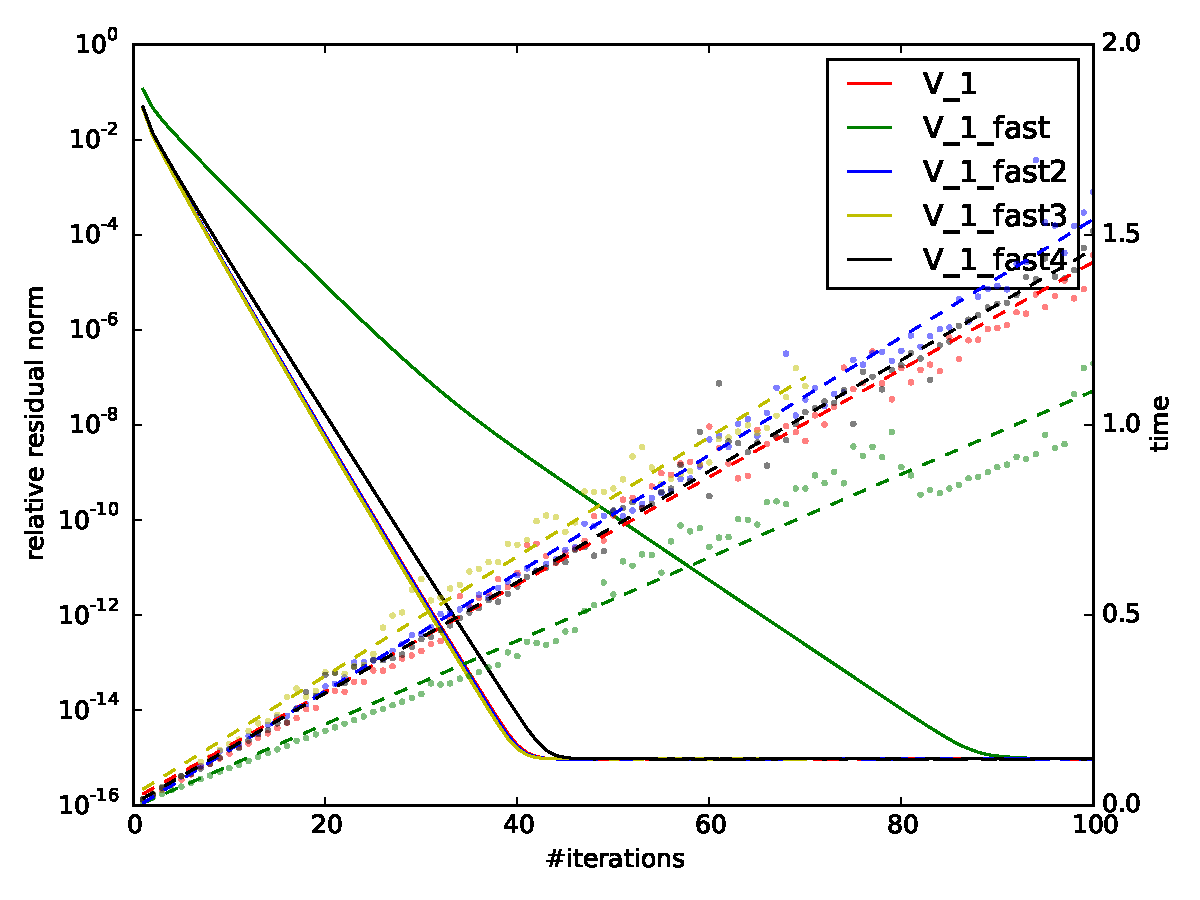
\includegraphics[width=0.49\linewidth]{figs/convergence_fast_small.pdf}
   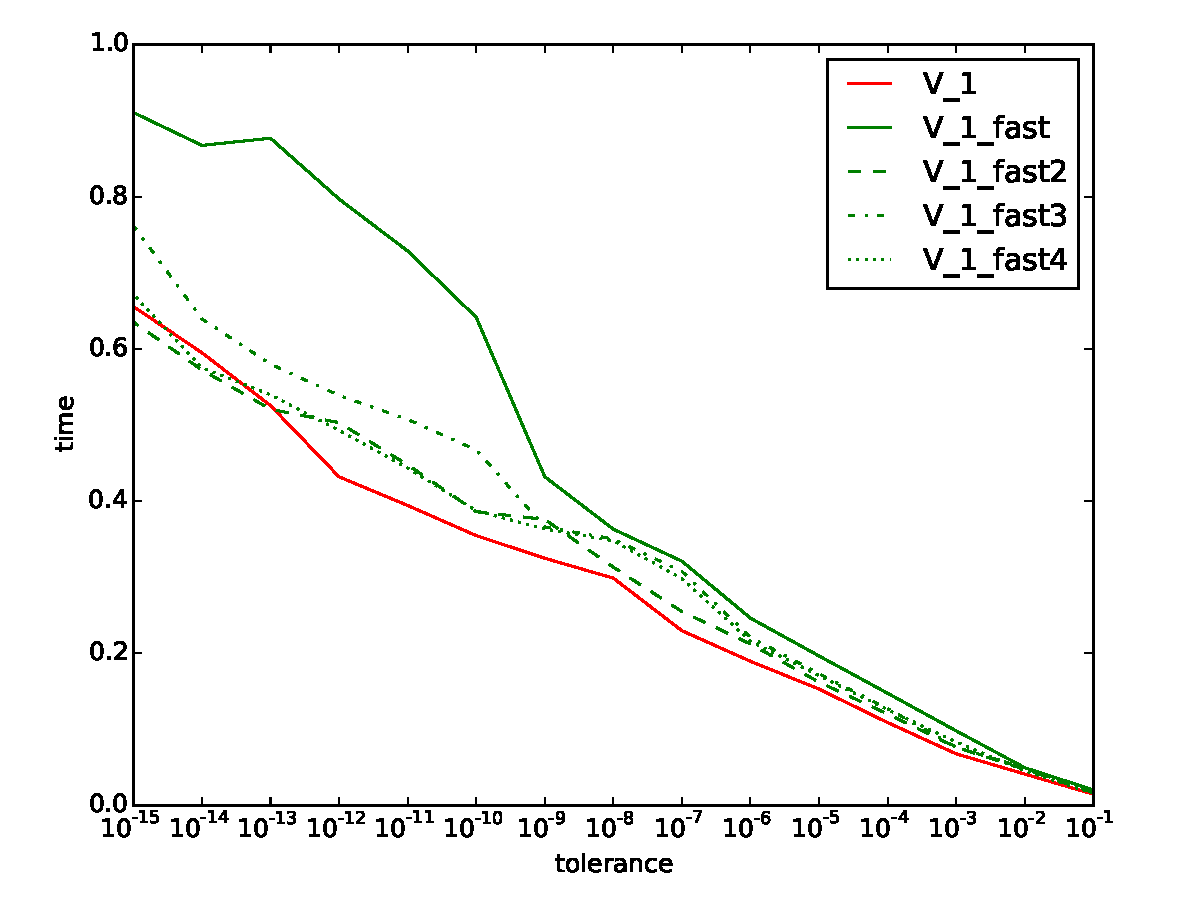
\includegraphics[width=0.49\linewidth]{figs/time_convergence_fast_small.pdf}
   \caption{Execution time and final residual norm for the 4 new strategies on a small matrix.}
   \label{fig.newstrat_small}
  \end{figure}

  The first thing to observe is that removing the relaxation at level 1 is a disaster. It sure saves time during a cycle but the accuracy loss is tremendous.
  The other thing to notice is that adding a lot of relaxations in the last levels increases by a little the execution time while being useless on the accuracy side. This is why \emph{Fast2} and  \emph{Fast3} are not really efficient.
  
  More tests were performed on the original $512,000\times 512,000$ and are presented in Figure~\ref{fig.newstrat}.
  
  \begin{figure}
  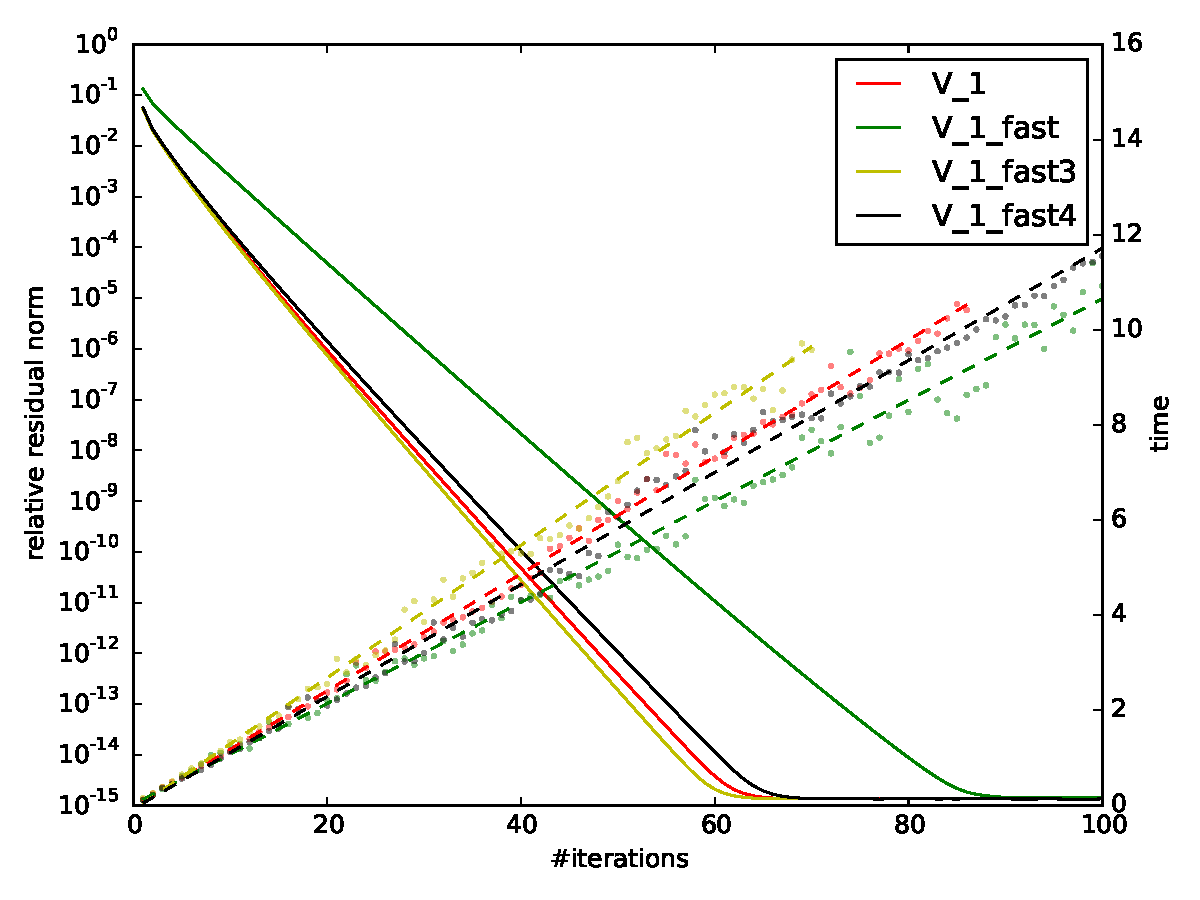
\includegraphics[width=0.49\linewidth]{figs/convergence_fast.pdf}
   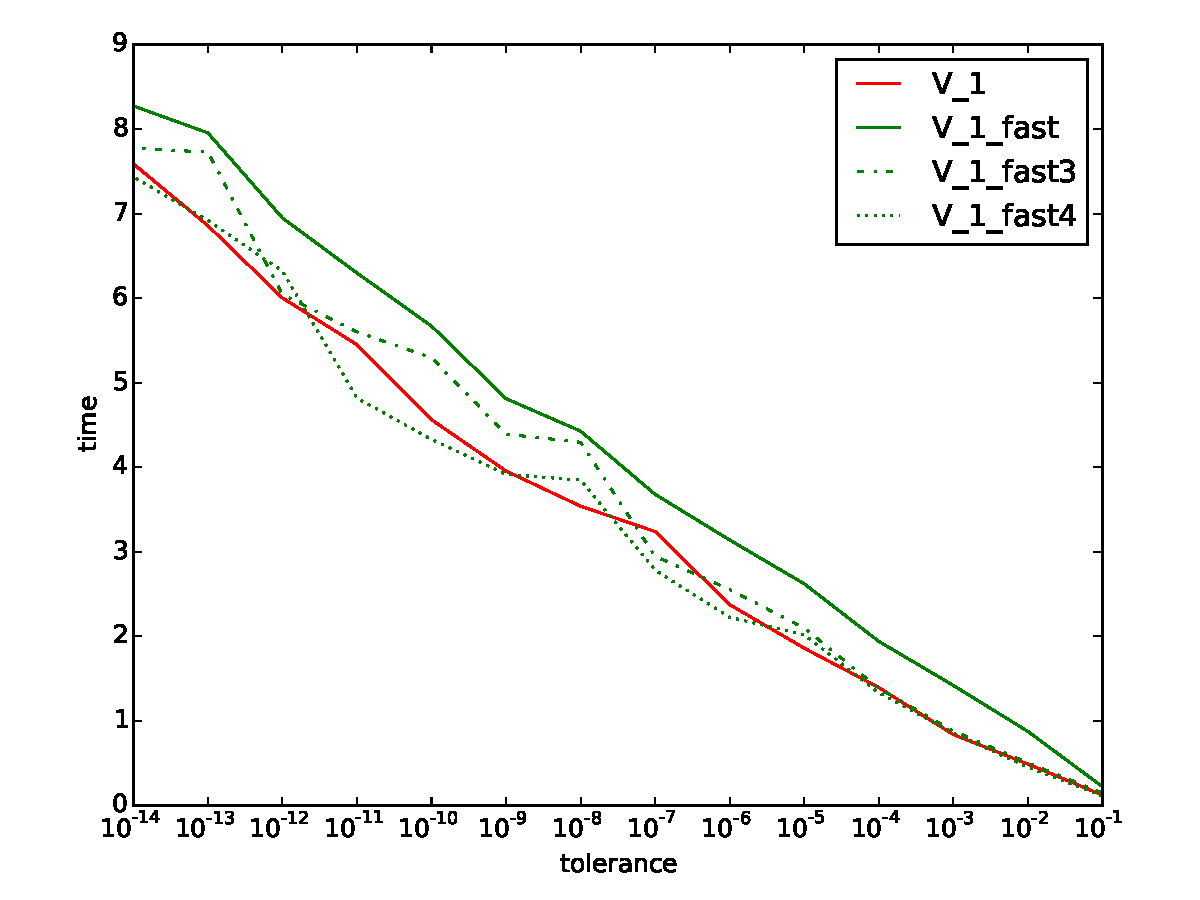
\includegraphics[width=0.49\linewidth]{figs/time_convergence_fast.pdf}
   \caption{Execution time and final residual norm for the 4 new strategies on the bigger matrix.}
   \label{fig.newstrat}
  \end{figure}
  
\subsection{An asymmetric strategy}
  We observe no big improvement compared to the original V-cycle with 1 relaxation at each level with the previous strategies.
  Their common point is that they all do the same number of relaxations when going down or up in the cycle. However, the main idea of the multi-grid is totally asymmetric.
  We first compute an approximation at a given level $l$, then we use the level $l+1$ to compute an approximate error term $e^l$ and finally we redo some relaxation to refine the solution. The two relaxations do not have the same goal.
  What if we could ensure that any value of error vector will be less than $\epsilon$ from the exact value? We would not need to do a relaxation
  before computing the approximate error term using the next levels in the grid. From that idea we define a new asymmetric strategy: we use a V-cycle with $\alpha_1 = 0$ and $\alpha_2 = 1$. In other words
  we do one relaxation at each level only when we are going up in the cycle. We call this strategy \emph{Up}.
  
  We run \emph{Up} and \emph{Fast4}, as long as the classical V-cycle, on the same matrix of size 512,000 and also on
  other applications (3D laplace with a 9-pt stencil, 3D laplace with a 27-point stencil, and another 3D partial derivative equation) with the same size of matrix.
  
  All results are presented in Figure~\ref{fig.up_comparison}.
  
  \begin{figure}
   \subfloat[Problem 1]{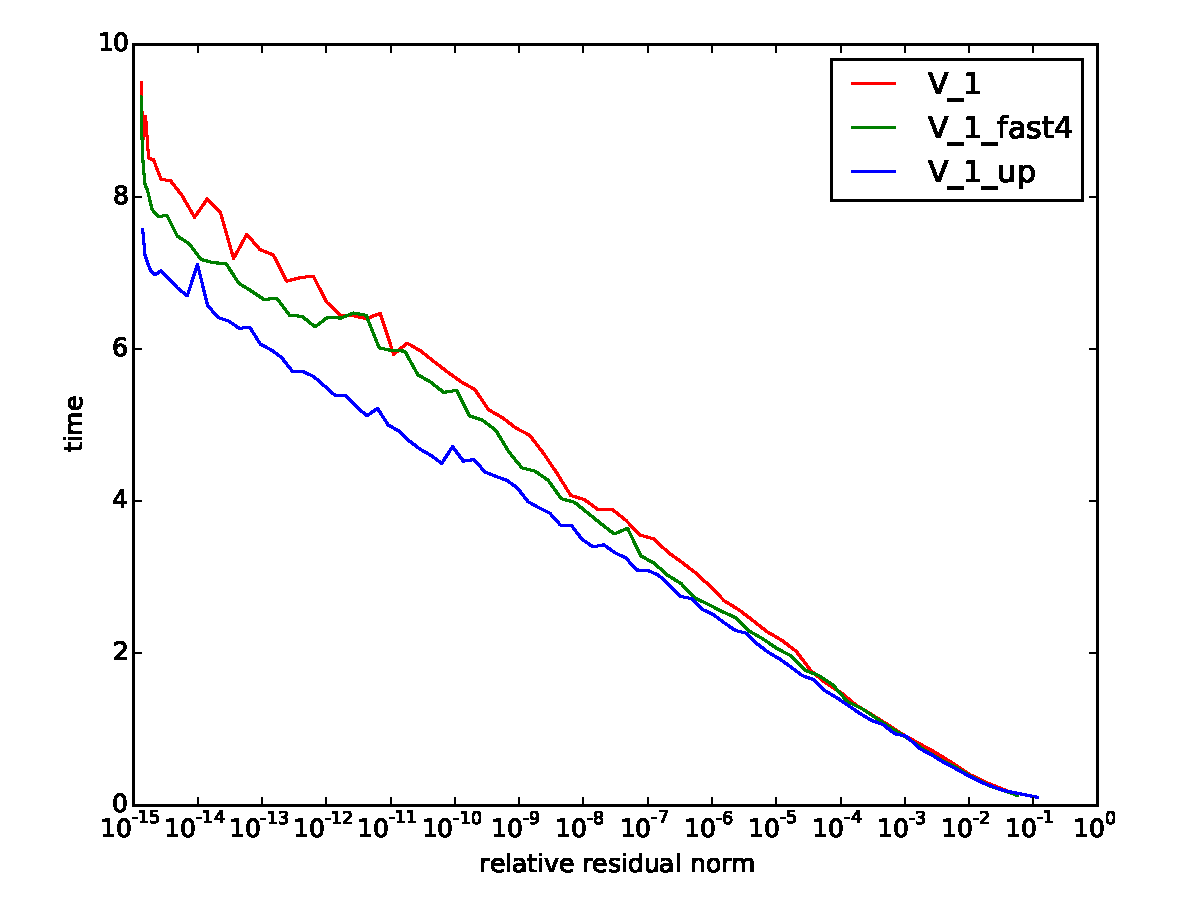
\includegraphics[width=0.49\linewidth]{figs/time_convergence_up_1.pdf}}
   \subfloat[Problem 2]{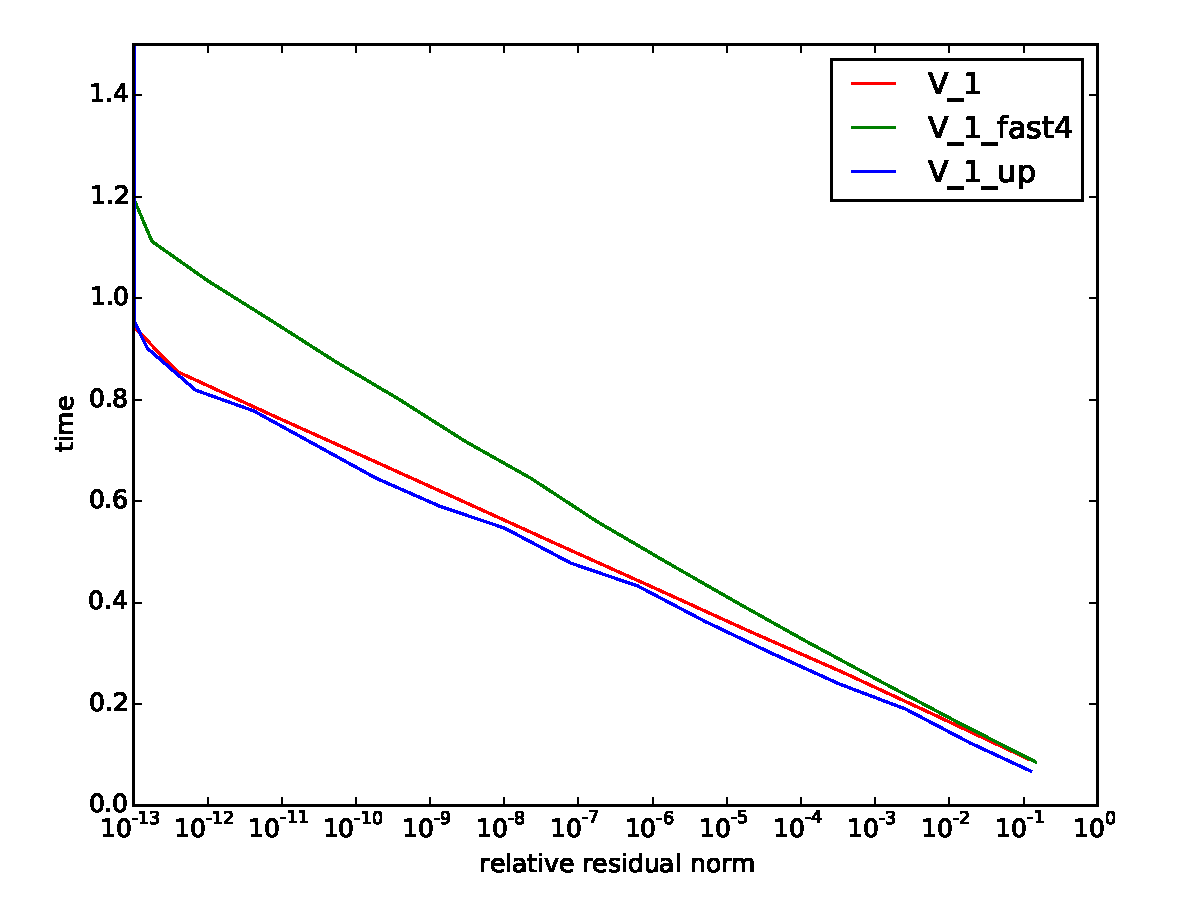
\includegraphics[width=0.49\linewidth]{figs/time_convergence_up_2.pdf}}\\
   \subfloat[Problem 3]{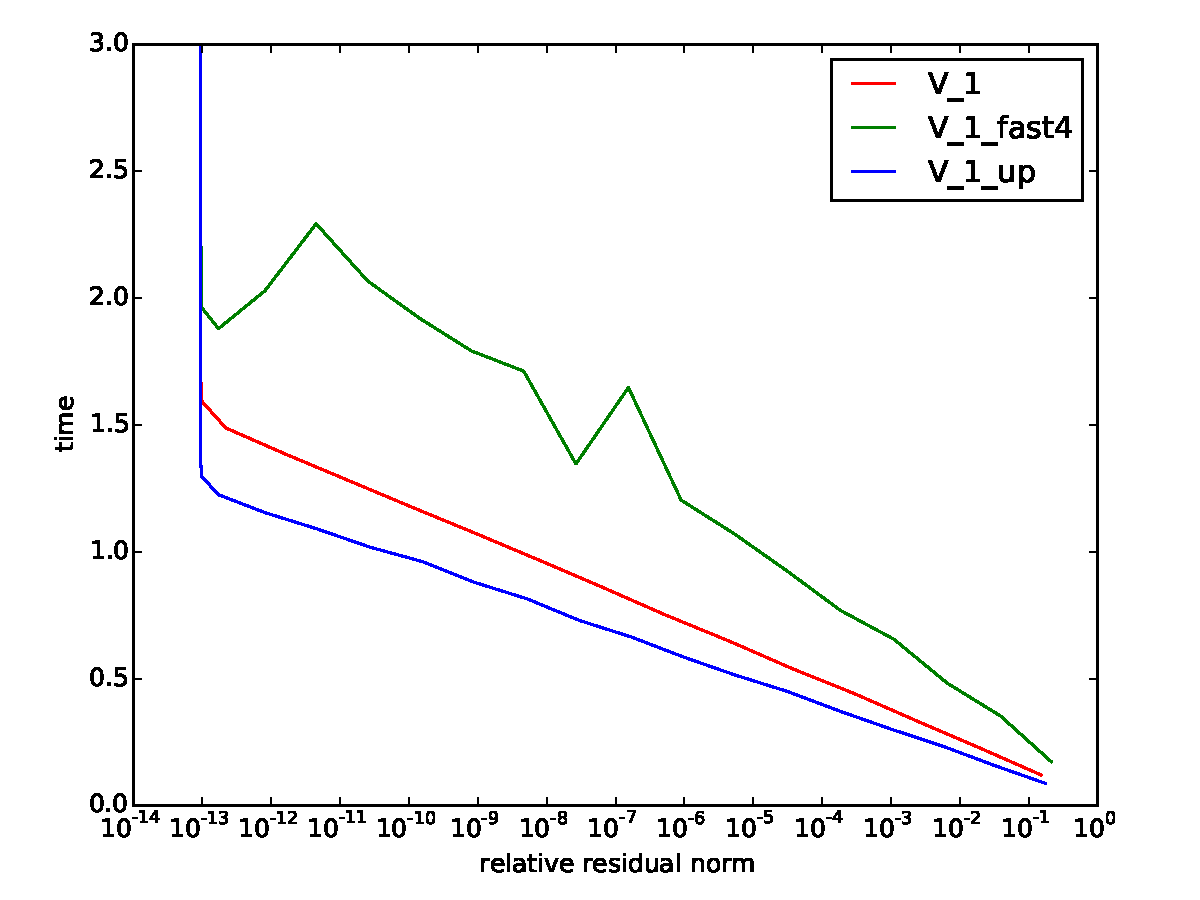
\includegraphics[width=0.49\linewidth]{figs/time_convergence_up_3.pdf}}
   \subfloat[Problem 4]{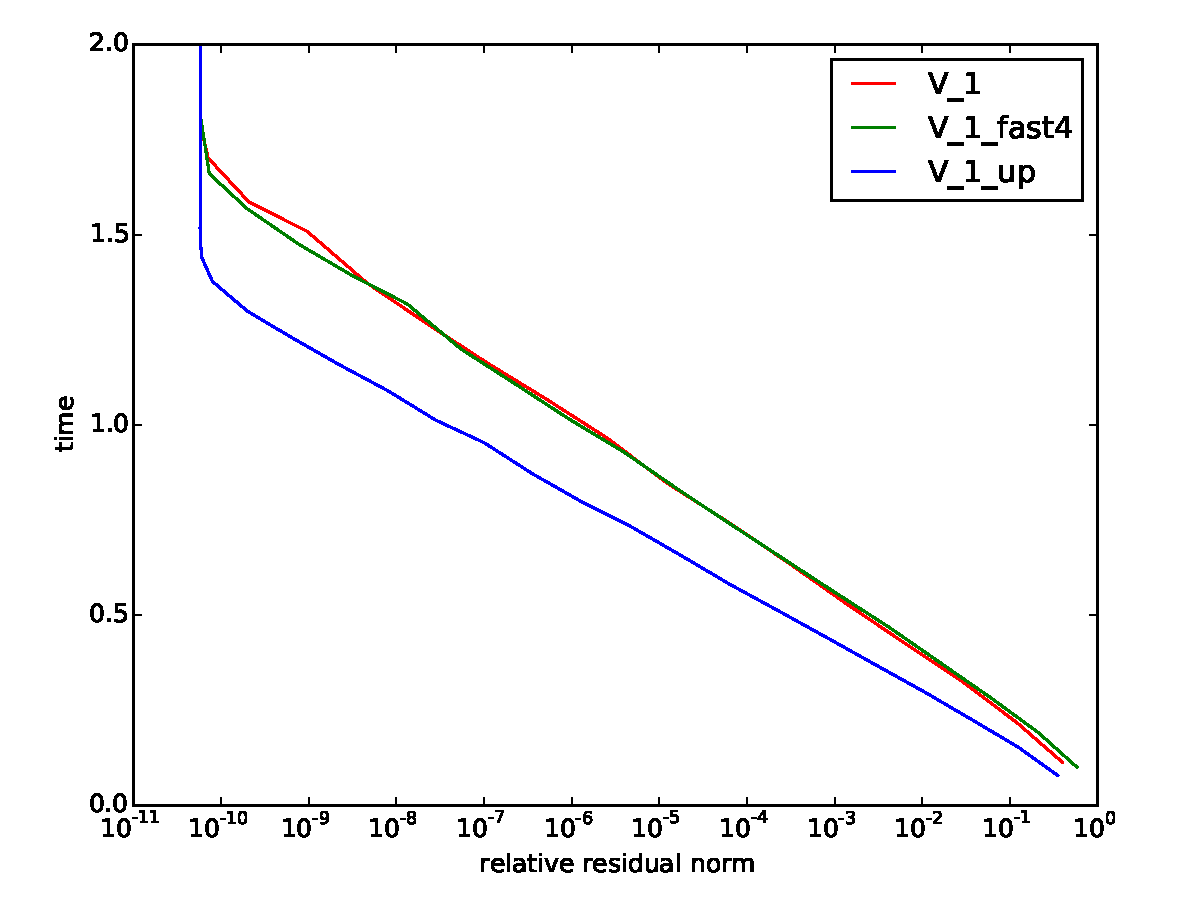
\includegraphics[width=0.49\linewidth]{figs/time_convergence_up_4.pdf}}
   \caption{Comparison of original algorithm with \emph{Fast4} and \emph{Up} strategies.}
   \label{fig.up_comparison}
  \end{figure}

   At this point, we see that it is not worth considering the \emph{Fast4} strategy anymore. However, \emph{Up} seems to be
   quite efficient since it improves by $12\%$,$7\%$,$20\%$ and $22\%$ (for problems 1,2,3 and 4 respectively) the average time needed to reach
   a $10^{-i}$ precision.
   However all these runs are sequential and does not guarantee the viability of the \emph{Up} strategy when the algorithm is parallelized.
   More tests were performed on MinoTauro with bigger matrices and different processor topologies. The total size of the matrix is set to either
   5,832,000 or 13,824,000, while the topology will be composed of either 27 (3x3x3), 36 (6x6x1) or 64 (4x4x4) processors.
   The problems tested were the problem 2 and the problem 3 (Laplace equation with either 9 or 27 points stencil).
   For these 6 possible combinations, we observe an averaged improvement of 18.4\% (ranging from 16.0\% to 28.3\%) for problem 2 and 20.5\% (ranging from 16.2\% to 25.0\%) for problem 3. It seems that \emph{Up} outperforms
   even more the classical V-cycle when the problem size increases, but seems to cap at around 25\% improvement. Figure~\ref{fig.mtup} presents the results for the matrix size 13,824,000 and problem 3, for the 3 different processor topologies. We have similar figures
   for the other scenarios.
   
   \begin{figure}
    \subfloat[3x3x3]{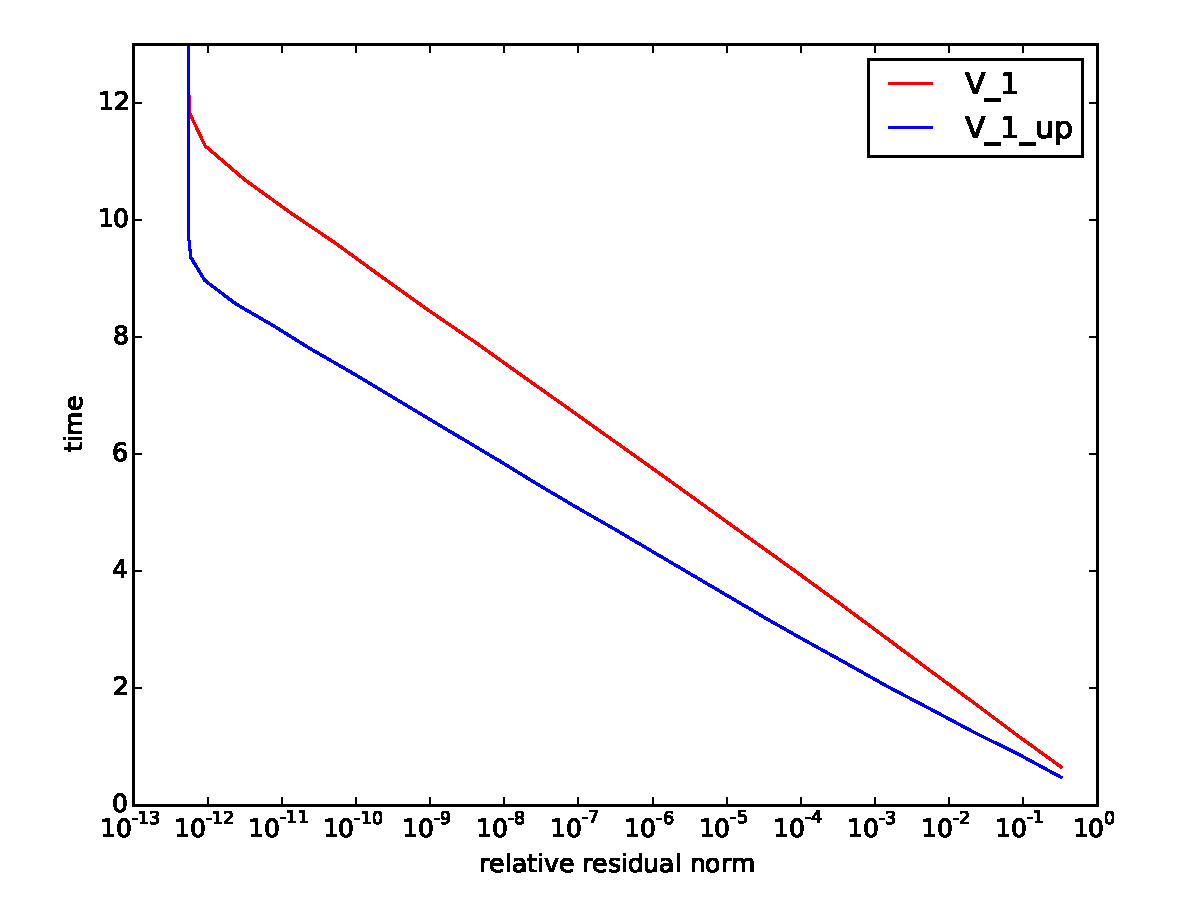
\includegraphics[width=0.33\linewidth]{figs/mt_27.pdf}}
    \subfloat[4x4x4]{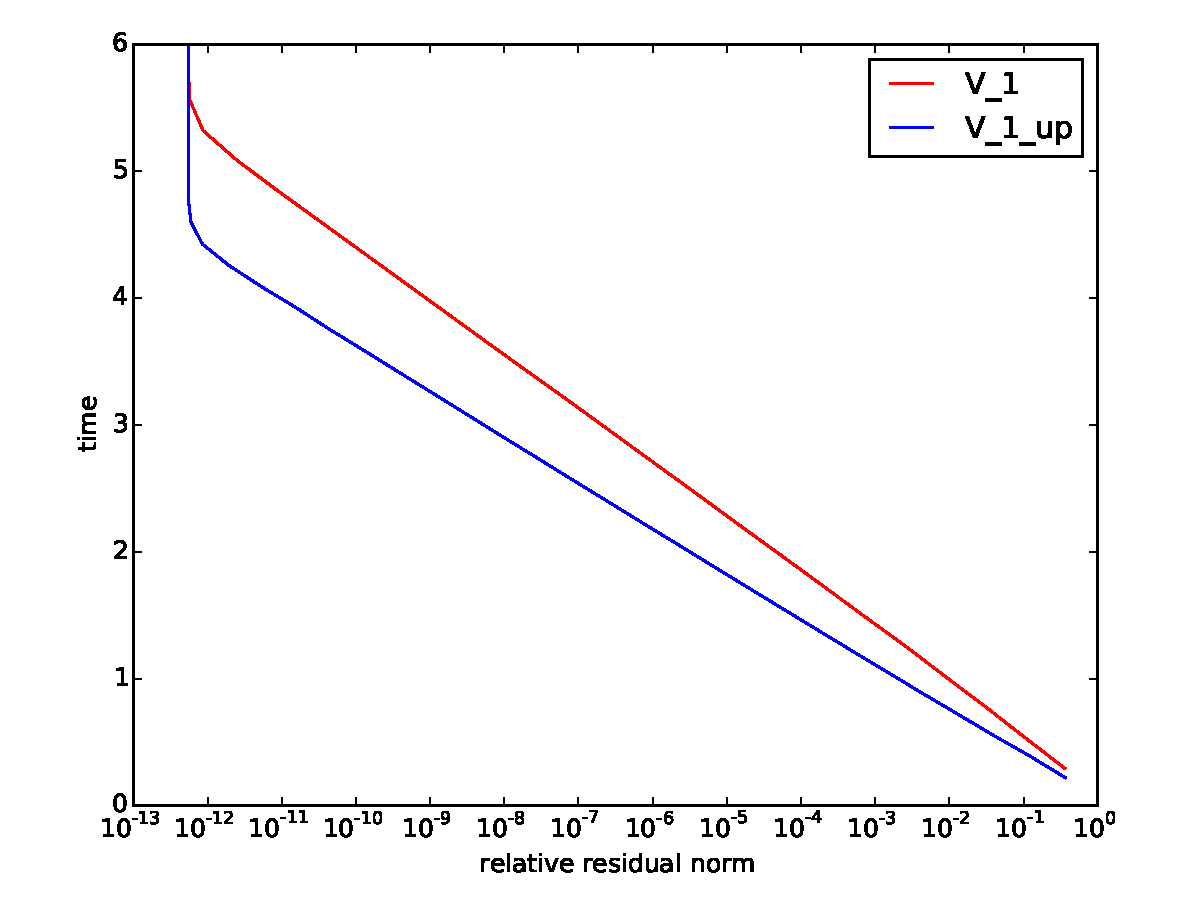
\includegraphics[width=0.33\linewidth]{figs/mt_64.pdf}}
    \subfloat[6x6x1]{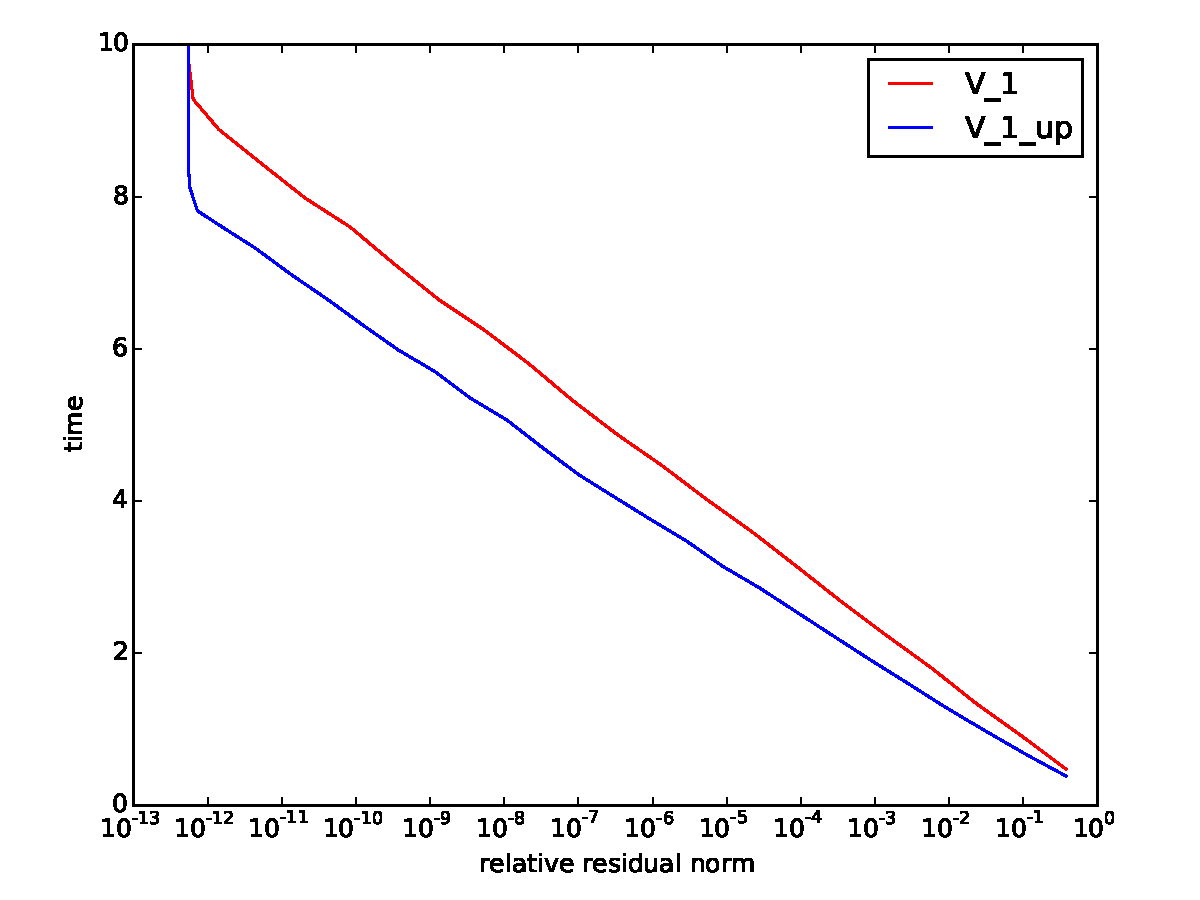
\includegraphics[width=0.33\linewidth]{figs/mt_36.pdf}}
    \caption{Comparison of original algorithm with \emph{Up} strategy for Laplace problem with 27-point stencil on a 240x240x240 grid.}
    \label{fig.mtup}
   \end{figure}

   \section{Playing with bits}
   
   If we look at the previous section, we see that we have a lower bound (which depends on the topology and the problem considered) on the accuracy we can achieve. This bound comes from the internal limitations of the \texttt{double} type.
   Indeed, a double uses 8 bytes (52 bits for the mantissa, 11 for the exponent and 1 bit for the sign). This representation does not allow a full description of all rational numbers (for exemple between $2^{52} and 2^{53}$ only integers can be represented).
   If we increase the number of bits of the mantissa or the exponent we can describe more and more numbers. In the other way, if we reduce it, we lose accuracy for numbers that are not representable. Considering our algorithm, what if we only want
   a precision of only $10^{-3}$ ? We don't need the 64 bits of a \texttt{double}, to reach it, a smaller number is enough. The advantage of using less bits for the floating point numbers is a faster and energy-saving computation. Thus it is important
   to study the impact of using a representation with smaller mantissa.
   
   To realize these experiments, we use two modified versions of the original algorithm. We modify the function that does the relaxation step (remember it is the costly part of the whole algorithm).
   In this function we can find different internal variables that originally of type \texttt{double}: 5 arrays and 8 scalars. The first version, \emph{AMGfloat}, changes the type of these 13 variables from \texttt{double*} or \texttt{double}
   to \texttt{float*} or \texttt{float}. For the second version, we use the library MPFR~\cite{MPFR,MPFR_link} that introduces a type \texttt{mpfr\_t}. This type has a parameter which is the number of bits in the mantissa of the variable.
   Every computation is done exactly (assuming the inputs are exact) then rounded to a number using exactly the number of bits set as parameter. We build the second version, \emph{AMGmpfr(b)}, by replacing only the 8 scalar variables
   by \texttt{mpfr\_t} variables, all using the same number of $b$ bits for the mantissa. In terms of arithmetic precision, \emph{AMG} behaves similarly to \emph{AMGmpfr(53)} and \emph{AMGfloat} to \emph{AMGmpfr(24)}. There can be small differences
   due to the rounding method used.
   
   The Figure~\ref{fig.bits_accuracy} represent the accuracy we reach using either \emph{AMGmpfr(8)}, \emph{AMGmpfr(16)}, \emph{AMGfloat}, \emph{AMGmpfr(32)} or \emph{AMGmpfr(64)}. The problem is problem 1, with 2x2x2 processor topology and 20x20x20 matrix size.
   What we actually see on this figure is the threshold reachable depending on the number of bits used. However, until this threshold is reach, the accuracy obtained using any number of bits is the same. This means that, for example,
   while the accuracy of the solution is below the threshold using 32 bits, using 32 or any greater number of bits to do the computations will result in the same final accuracy. However, we expect that using only the necessary $32$ bits is 
   more efficient in terms of time, space and energy.
   
   \begin{figure}
   % 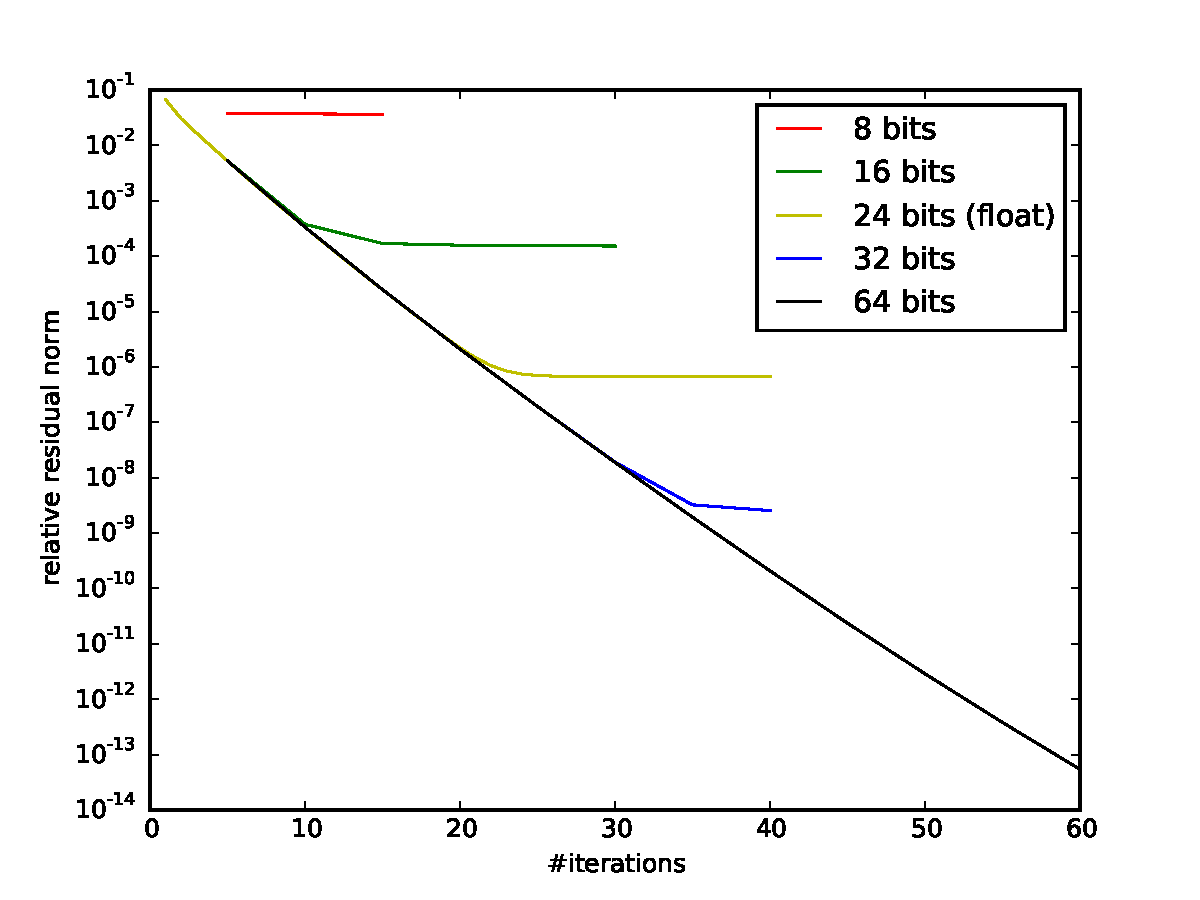
\includegraphics[width=0.8\linewidth]{figs/bits_convergence.pdf}
    \caption{Accuracy achievable with different number of bits in mantissa.}
    \label{fig.bits_accuracy}
   \end{figure}
   
   The second thing to see is that \emph{AMGfloat} behaves exactly as \emph{AMGmpfr(24)} in terms of accuracy whereas more variables were changed from \texttt{double} to \texttt{float}. It does not degrade more the accuracy, only a few variables
   from the 8 scalars actually control the final precision as they are temporary variables used for intermediate computations before being plugged back into the input matrix/vector.
   That being said, we design a new algorithm that adapts the precision of the variables during the execution. It is the same algorithm as \emph{AMGmpfr(b)} except this time the precision can change between two cycles.
   We fix a threshold on the ratio between the relative residual norm at two consecutive steps to trigger the precision change.
   Figure~\ref{fig.prec_incr} presents the evolution of accuracy for the original algorithm, and 3 different strategies with increasing precision and threshold of 0.8: start at $b=16$ and do $b=b+8$, start at $b=32$
   and do $b=b+8$, and start at $b=16$ and do $b=b\times2$, run on a 24Ox240x240 matrix size with 3x3x3 topology for problem 3.
   
   \begin{figure}
%    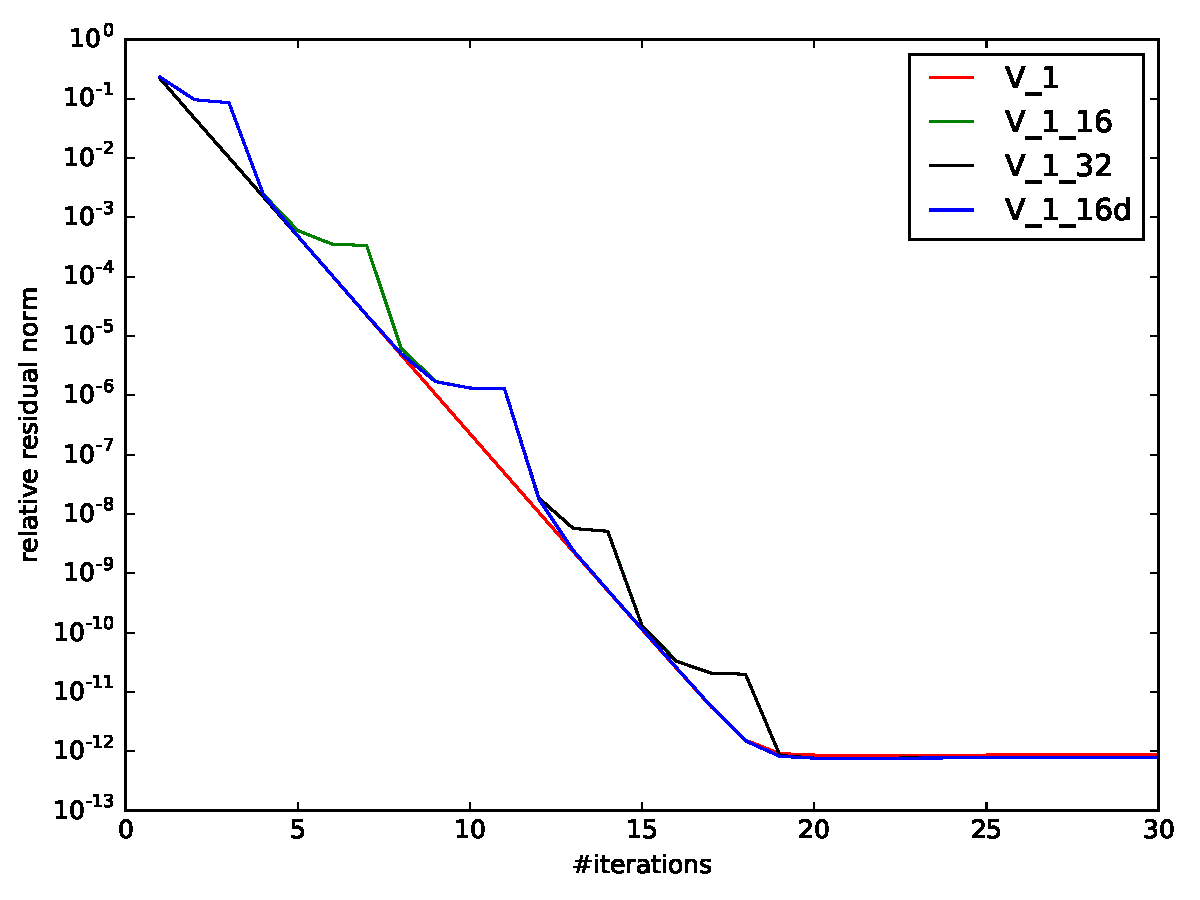
\includegraphics[width=0.8\linewidth]{figs/prec_incr.pdf}
    \caption{Accuracy of adaptive algorithms compared to the original double-precision.}
    \label{fig.prec_incr}
   \end{figure}
   
   We see some steps appear, corresponding to the lower bound on the accuracy at the current precision. Then the precision is adapted to be able to improve the overall accuracy. Even if we lose some accuracy by waiting for the ratio
   between two consecutive relative residual norm to be higher than the threshold, when the precision changes, the gain is more important than that of the original algorithm (i.e. the slope is bigger on the figure), which makes any of
   the 3 versions able to reach the maximum accuracy (of $4.7\times 10^{-13}$) in the same number of cycles as the original algorithm (20-21 cycles).
   
   Two questions arise at this step. How to evaluate the energy/time savings of this adaptive algorithm? Which precisions should be used to optimize these savings?\\
   The first question is not simple because the use of the MPFR library to do these accuracy experiments introduce a huge overhead in the computations (running \emph{AMGmpfr(53)} is about 20 times longer than running \emph{AMG} whereas it
   represents the final same algorithm), and this overhead is not highly influenced by the choice of the number of bits. Thus it is impossible just to measure the execution time of the algorithm using MFPR library.
   
   \subsection{Optimal set of precisions}
   
   \begin{theorem}
     Given $b_{max}$, a maximum number of bits, $n$ the number of different precisions $b_1,\dots,b_n$ to use, and $T(b)=\alpha b+c$, with $\alpha$ and $c$ two constants, the time to execute a cycle at precision $b$, then
     the execution time of our adaptive algorithm is minimized for $b_i = \frac{i}{n}b_{max}$.
   \end{theorem}

   \begin{proof}
   From the previous experiments we can see that (i) the number of cycles needed to reach the lower bound for a given precision does not depend on the previous cycles (Figure~\ref{fig.prec_incr}) and that (ii) the number of cycles
   needed to reach the lower bound is proportional to the number of bits $b$ used (Figure~\ref{fig.bits_accuracy}). We then define $\textsc{MaxIter}(b)$ the number of cycles needed so that the ratio between two consecutive
   relative residual norms is higher than a threshold $t$. We use the two observations to model $\textsc{MaxIter}(b) = \lfloor kb \rfloor$ for some constant $k$.
   Then we can compute the total execution time of the algorithm \[T_{total} = \textsc{MaxIter}(b_1)T(b_1) + \sum\limits_{i=1}^{n-1} (\textsc{MaxIter}(b_{i+1})-\textsc{MaxIter}(b_i))T(b_{i+1}). \]
   Indeed, when we reach the number of iterations $\textsc{MaxIter}(b_i)$ we change from precision $b_i$ to precision $b_{i+1}$.
   We can rewrite $T_{total}$ as
   \begin{align*}
    T_{total} &\approx k b_{1} T(b_1) + \sum\limits_{i=1}^{n-1} k(b_{i+1}-b_{i})T(b_{i+1})\\
	    & \approx k ( b_{n}T(n) + \sum\limits_{i=1}^{n-1} b_i ( T(b_i) - T(b_{i+1})).
   \end{align*}
   By plugging the expression of $T(b)$ into the previous equation and considering the maximum precision we want is $b_{max}=b_n$, we finally get:
   \begin{equation}
    T_{total}  = k\alpha\left(b_n^2 + \sum\limits_{i=1}^{n-1} (b_i^2 - b_i b_{i+1})\right) + kb_{max}c.
   \end{equation}
   
   Let us consider the function $f(x_1,\dots,x_n) = \sum\limits_{i=1}^n x_i^2 - \sum\limits_{i=1}^{n-1} x_ix_{i+1}$. Finding the minimum of $f(x_1,\dots,x_{n-1},1)$ will give
   us the minimum of the execution time.
   By simple partial derivation:
   \[ \frac{\partial f(x_1,\dots,x_n)}{\partial x_i} = 2x_i - (1-\delta_{i,n})x_{i+1} - (1-\delta_{i,1})x_{i-1} \]
   where $\delta_{a,b} $ is equal to 1 if and only if $a=b$, 0 otherwise.
   
   This is where the boundary condition $x_n = 1$ is useful: if we do not set it to a number different from 0, the function is minimized for $x_1=\dots=x_n=0$. This applied to our problem
   has no sens, as we would't be doing any computation. The boundary condition represents the fact that we need to reach a existing precision ($b_{max}$) eventually. By a simple scaling,
   considering $1$ instead of $b_{max}$ makes computation easier and does not change the resolution of the the following system (up to a factor):
   
   \resizebox{0.9\linewidth}{!}{
   $\left\{
   \begin{tabular}{rcl cccccccccc cl}
    $\frac{\partial f(x_1,\dots,x_n)}{\partial x_1}$ & = & $2x_1$ & $-$ & $x_2$  &     &       & & 	 &&     &     &       & = & 0 \\
    $\frac{\partial f(x_1,\dots,x_n)}{\partial x_2}$ & = & $-x_1$ & $+$ & $2x_2$ & $-$ & $x_3$ & & 	 &&     &     &       & = & 0 \\
    & \vdots &&&&&&&&&&&&&\\
    $\frac{\partial f(x_1,\dots,x_{n})}{\partial x_{n-1}}$ & = &        &     &        &     &       & & $-x_{n-2}$ & $+$ & $2x_{n-1}$ & $-$ & $x_n$ & = & 0 \\
    $x_n$ & = & 1 &&&&&&&&&&&&\\
   \end{tabular} \right.$
  }
  
  Solving this system of equations is equivalent to solving the linear system $Ax=b$ where
  \[ A = \begin{bmatrix}
    2       & -1 &  &  &  \\
    -1       & 2 & -1 &  &  \\
    & \ddots & \ddots & \ddots & \\
    & & -1 & 2 & -1 \\
           &  &  & -1 & 2
\end{bmatrix} \textup{ and } b = \begin{bmatrix} 0 \\ \vdots \\ 0 \\ 1 \end{bmatrix} \]
   
   This system has a unique solution which is $\begin{bmatrix} \frac{1}{n} & \dots & \frac{n-1}{n} \end{bmatrix}$.
   The minimum of $f(x_1,\dots,x_n)$ with boundary condition $x_n=1$ is thus reached for $x_i = \frac{i}{n}$.
   It is, when multiplied by $b_{max}$, the solution that minimizes our total execution time.
   \end{proof}
   
   P1x1x1, 10 iterations, average on ten runs\\
   \begin{tabular}{|l|c|c|c|c|}
   \hline
    \multirow{2}{*}{Experiment} & \multicolumn{2}{c|}{Single-Precision} & \multicolumn{2}{c|}{Double-precision} \\
    \cline{2-5}
    & Solve (s) & Cycle (ms) & Solve (s) & Cycle (ms) \\
    \hline
    (1) 40x40x40 & 1.308 & 12 & 1.543 & 14\\
    \hline
    (1) 80x80x80 & 10.794 & 100 & 13.033 & 121.5\\
    \hline
    (2) 20x20x20 & 0.1316 & 1.1 & 0.1411 & 1.2 \\
    \hline
    (2) 40x40x40 & 1.026 & 9.5 & 1.195 & 11 \\
    \hline
    (2) 80x80x80 & 8.068 & 74 & 9.595 & 88 \\
    \hline
     (3) 20x20x20 & 0.170 & 1.4 & 0.179 & 1.5 \\
    \hline
     (3) 40x40x40 & 1.396 & 11.5 & 1.646 & 13.7 \\
    \hline
     (3) 80x80x80 & 10.644 & 89 & 12.572 & 106 \\
    \hline
     (4) 20x20x20 & 0.1405 & 1.2 & 0.149 & 1.3 \\
    \hline
     (4) 40x40x40 & 1.192 & 11 & 1.402 & 15\\
    \hline
     (4) 80x80x80 & 10.258 & 96 & 12.125 & 114 \\
    \hline
   \end{tabular}	
   
   Jacobi\begin{tabular}{|l|c|c|c|c|}
   \hline
    \multirow{2}{*}{Experiment} & \multicolumn{2}{c|}{Single-Precision} & \multicolumn{2}{c|}{Double-precision} \\
    \cline{2-5}
    & Solve (s) & Cycle (ms) & Solve (s) & Cycle (ms) \\
    \hline
    (1) 40x40x40 & 0.0868 & 7.8 & 0.09577 & 8.4\\
    \hline
    (1) 80x80x80 & 0.709 & 63 & 0.8757 & 73\\
    \hline
    (2) 20x20x20 & 0.00945 & 0.8 & 0.00991 & 0.9 \\
    \hline
    (2) 40x40x40 & 0.0755 & 6.5 & 0.0815 & 7.2 \\
    \hline
    (2) 80x80x80 & 0.581 & 51 & 0.648 & 57 \\
    \hline
     (3) 20x20x20 & 0.0121 & 0.95 & 0.0126 & 1.0 \\
    \hline
     (3) 40x40x40 & 0.0990 & 7.8 & 0.105 & 8.2 \\
    \hline
     (3) 80x80x80 & 0.759 & 60 & 0.878 & 75 \\
    \hline
     (4) 20x20x20 & 0.0104 & 0.92 & 0.0106 & 1.0 \\
    \hline
     (4) 40x40x40 & 0.0842 & 7.6 & 0.0972 & 8.8\\
    \hline
     (4) 80x80x80 & 0.720 & 64.5 & 0.810 & 75.5 \\
    \hline
   \end{tabular}

   (1) 64x64x64, 50 iterations, averaged on 10 runs\\
   \begin{tabular}{|l|c|c|c|c|}
   \hline
    \multirow{2}{*}{Experiment} & \multicolumn{2}{c|}{Single-Precision} & \multicolumn{2}{c|}{Double-precision} \\
    \cline{2-5}
    & Solve (s) & Cycle (ms) & Solve (s) & Cycle (ms) \\
    \hline
    1x1x1 & 4.382 & 70-80 & 5.76 & 80-90\\
    \hline
    2x1x1 & 2.638 & 40-50 & 3.091 & 50-60\\
    \hline
    2x2x1 & 1.659 & 30-40 & 2.511 & 40-50 \\
    \hline
    2x2x2 & 0.898 & 10-20 & 1.087 & 10-20 \\
    \hline
    4x2x2 & 0.302 & 0-10 & 0.568 & 10 \\
    \hline
    4x4x2 & 0.220 & 0-10 & 0.260 & 0-10 \\
    \hline
    4x4x4 & 0.252 & 0-10 & 0.315 & 0-10 \\
    \hline
   \end{tabular}
   
   (1) 64x64x64, 50 iterations, averaged on 10 runs\\
   \begin{tabular}{|l|c|c|c|c|}
   \hline
    \multirow{2}{*}{Experiment} & \multicolumn{2}{c|}{Single-Precision} & \multicolumn{2}{c|}{Double-precision} \\
    \cline{2-5}
    & Solve (s) & Cycle (ms) & Solve (s) & Cycle (ms) \\
    \hline
    1x1x1 & 2.627 & 40-50 & 3.895 & 50-60\\
    \hline
    2x1x1 & 1.730 & 30 & 2.575 & 40-60\\
    \hline
    2x2x1 & 1.079 & 20 & 1.588 & 30-40 \\
    \hline
    2x2x2 & 0.560 & 10 & 0.847 & 10-20 \\
    \hline
    4x2x2 & 0.217 & 0-10 & 0.273 & 0-10 \\
    \hline
    4x4x2 & 0.181 & 0-10 & 0.201 & 0-10 \\
    \hline
    4x4x4 & 0.224 & 0-10 & 0.258 & 0-10 \\
    \hline
   \end{tabular}
   \bibliography{biblio}
   \bibliographystyle{plain}
\end{document}
